\documentclass[a4paper, 11pt]{article}
\usepackage[bottom=2cm,top=3cm,left=2.5cm,right=2.5cm]{geometry}
\usepackage[utf8]{inputenc}
\usepackage[T1]{fontenc}
\usepackage[portuguese]{babel}
\usepackage{graphicx}
\usepackage{indentfirst}
\usepackage{float}
\usepackage{fancyhdr}
\usepackage{booktabs}
\usepackage{multirow}
\usepackage{setspace}
\usepackage{amsmath}
\usepackage{amssymb}
\usepackage{subcaption}
\usepackage{xcolor}
\usepackage{listings}
\usepackage{tikz}
\usetikzlibrary{positioning, arrows.meta, fit, backgrounds, calc}
\usepackage[hidelinks]{hyperref}

\hypersetup{
    colorlinks=true,
    linkcolor=blue,
    filecolor=magenta,
    urlcolor=cyan,
    citecolor=blue,
}
\urlstyle{same}

% Cabeçalho/rodapé da disciplina.
\pagestyle{fancy}
\lhead{\textsc{Teleinformática e Redes 1}}
\rhead{\textsc{
\includegraphics[height=25pt]{unb1}}}
\renewcommand{\headrulewidth}{0.4pt}
\renewcommand{\footrulewidth}{0.4pt}
\setlength\headheight{30pt}

% Estilo para trechos de código curtos.
\lstset{
    basicstyle=\ttfamily\footnotesize,
    breaklines=true,
    columns=fullflexible,
    keepspaces=true,
}

% Caixa reservada para o grupo colar as capturas dos gráficos depois.
\newcommand{\placeholdergrafico}[2]{%
    \fbox{\begin{minipage}[c][#1][c]{0.95\linewidth}\centering
    \textcolor{gray}{\textit{[Espaço reservado para o gráfico: #2]}}
    \end{minipage}}%
}

\begin{document}

% ==================================================================
%  CAPA
% ==================================================================
\begin{titlepage}
 \vfill
  \begin{center}
  
\includegraphics[scale=0.5]{UNB.png}\\[6pt]
   {\large \textbf{Universidade de Brasília}} \\
   {\large \textbf{Departamento de Ciência da Computação}} \\
   {\large \textbf{Teleinformática e Redes 1 --- CIC0235}} \\

   \vfill

   \Large{\textbf{Simulador TR1 --- Camadas Física e de Enlace}}\\

   \vfill
   \vspace{40pt}

   \begin{center}
   \large{Anna Luiza Novaes Jansen Silva --- 232024572}\\[2pt]
   \large{João Pedro Borges Saraiva --- 231025280}\\[2pt]
      \large{Luís Eduardo Curi Serra --- 251033574}\\\vfill
   \textbf{\LARGE{Professor: Marcelo Antonio Marotta}}\\
   \end{center}

   \vfill
   \textbf{\today}
  \end{center}
\end{titlepage}
\newpage

\setlength\parindent{18pt}
\setstretch{1.02}

% ==================================================================
%  1. INTRODUÇÃO
% ==================================================================
\section{Introdução}

O objetivo deste trabalho é \textbf{simular as camadas Física e de Enlace} de uma rede de
computadores, reproduzindo o caminho de uma mensagem de texto desde a digitação no
\textbf{transmissor (TX)} até a sua recuperação no \textbf{receptor (RX)}. O problema central
é representar a informação como \emph{sinal elétrico},
transmiti-lo por um meio que insere \textbf{ruído gaussiano} e, ainda assim, recuperar a
mensagem original por meio dos protocolos de enquadramento, detecção e correção de erros.

O simulador foi desenvolvido em \textbf{Python 3}, sem bibliotecas prontas para os algoritmos
centrais (CRC, Hamming, modulações): \texttt{NumPy} e \texttt{Matplotlib} são usados apenas
para manipular vetores e plotar sinais~\cite{numpy,matplotlib}. O fluxo completo é:

\begin{center}
\small
texto $\rightarrow$ bits $\rightarrow$ Enlace (EDC/ECC + enquadramento) $\rightarrow$
Física (sinal V/W) $\rightarrow$ \fbox{meio com ruído $n(x,\sigma)$} $\rightarrow$
Física RX $\rightarrow$ Enlace (desenquadramento + EDC/ECC) $\rightarrow$ bits $\rightarrow$ texto.
\end{center}

Em conformidade com a Figura~1 o TX e o RX são
\textbf{processos separados}, executados como duas janelas gráficas independentes que se
comunicam por um \textbf{socket TCP local}, o qual representa o meio de comunicação onde o
ruído é aplicado.

% ==================================================================
%  2. IMPLEMENTAÇÃO
% ==================================================================
\section{Implementação}

\subsection{Organização e arquitetura}

O código foi modularizado em arquivos
(Tabela~\ref{tab:arquitetura}). A comunicação entre camadas usa uma convenção única de dados:
\textbf{bits} são listas de inteiros \texttt{0/1} (\texttt{list[int]}); o \textbf{sinal} é um
\texttt{np.ndarray} de valores reais em V/W, com tensão alta $V_+ = 1,5V$, \texttt{AMOSTRAS\_POR\_BIT = 100} amostras por
bit/símbolo e frequência base $f=2Hz$, quando aplicavel. Para a interface escolher as 
técnicas em tempo de execução, cada camada expõe
\textbf{despachantes} que mapeiam a string da GUI para a implementação correspondente,
\texttt{coder}/\texttt{decoder} e \texttt{modulator}/\texttt{demodulator} na física.

No enlace o tamanho do cabeçalho é fixo em 16 bits para a contagem de caracteres, 
o tamanho máximo do quadro é fixado em 212 bits e mínimo de 4 bits, o polinômio do CRC-32 é $0x04C11DB7$, 
por fim, de forma equivalente a camada física
são utilizados modulos de seleção \texttt{adicionar\_controle\_erro} 
e \texttt{aplicar\_enquadramento}, vale ressaltar que por simplicidade das implementações seguintes
o código aceita apneas aplicar EDC ou ECC no sinal, não sendo contemplada a possibilidade
de utilizar os dois no mesmo sinal. 

Ainda no GUI, é fixado uma representação máxima do sinal dos 40 primeiros bits recuperados, 
e a modulação por portadora prevalece sobre as configurações da modulação digital.


\begin{table}[H]
\centering
\small
\begin{tabular}{@{}ll@{}}
\toprule
\textbf{Arquivo} & \textbf{Responsabilidade} \\
\midrule
\texttt{CamadaFisica.py}     & Modulação digital, por portadora, amostragem e ruído. \\
\texttt{CamadaEnlace.py}     & Enquadramento, detecção (EDC) e correção (ECC) de erros. \\
\texttt{Transmissor.py}      & Fluxo TX: texto $\rightarrow$ bits $\rightarrow$ enlace $\rightarrow$ física. \\
\texttt{Receptor.py}         & Fluxo RX: sinal $\rightarrow$ física $\rightarrow$ enlace $\rightarrow$ texto. \\
\texttt{InterfaceGrafica.py} & GUI GTK 3 + Matplotlib (TX e RX). \\
\texttt{Simulador.py}        & Rotina que simula chamadas TX $\rightarrow$ meio $\rightarrow$ RX. \\
\texttt{utils.py}            & Conversões base (int$\leftrightarrow$bits, texto$\leftrightarrow$bits, padding, fatiar payload). \\
\bottomrule
\end{tabular}
\caption{Organização dos módulos do simulador.}
\label{tab:arquitetura}
\end{table}

\begin{figure}[H]
\centering
\resizebox{\textwidth}{!}{%
\begin{tikzpicture}[
  font=\scriptsize,
  >={Stealth[length=2mm]},
  camada/.style={draw, rounded corners=2pt, fill=white, align=center,
                 text width=3cm, minimum height=1.15cm, inner sep=3pt},
  config/.style={draw, rounded corners=3pt, fill=gray!12, align=center,
                 text width=12.6cm, inner sep=5pt},
  meio/.style={draw, rounded corners=3pt, fill=gray!18, align=center,
               text width=2.7cm, minimum height=4.9cm, inner sep=4pt},
  proc/.style={draw, dashed, rounded corners=5pt, inner sep=10pt},
  seta/.style={->, thick},
  setatrace/.style={->, thick, dashed},
  titulo/.style={font=\scriptsize\bfseries}
]

% ---------- Configuração geral (topo, compartilhada) ----------
\node[config] (cfg) at (5,3.2) {%
  \textbf{Configuração geral (Interface gráfica)}\\[1pt]
  Tam.\ máx.\ de quadro (212 bits, múltiplo de 8) $\cdot$ Tam.\ do EDC (\emph{checksum}) $\cdot$
  Enquadramento (contagem de caracteres / inserção de bytes / inserção de bits) $\cdot$
  Detecção \emph{ou} correção (paridade / checksum / CRC-32 / Hamming) $\cdot$
  Modulação digital (NRZ-Polar / Manchester / Bipolar) $\cdot$
  Modulação por portadora (ASK / FSK / PSK / QPSK / 16-QAM) $\cdot$
  Ruído: média $x$, desvio $\sigma$%
};

% ---------- Coluna TX (fluxo de cima para baixo) ----------
\node[camada] (txapp) at (0,0)    {\textbf{Aplicação de rede}\\ entrada de texto $\rightarrow$ texto em bits, fatiado em \emph{payloads} (até 212 bits)};
\node[camada] (txenl) at (0,-1.9) {\textbf{Camada de enlace}\\ adiciona EDC \emph{ou} ECC $\rightarrow$ enquadramento (por quadro)};
\node[camada] (txfis) at (0,-3.8) {\textbf{Camada física}\\ modulação por portadora \emph{ou} codificação banda-base $\rightarrow$ sinal em V/W};

% ---------- Meio de comunicação (canal) ----------
\node[meio] (meio) at (5,-1.9) {%
  \textbf{Meio de comunicação (canal)}\\[3pt]
  ruído gaussiano $n(x,\sigma)$ somado ao sinal (V/W) recebido do TX, antes do envio pelo TCP\\[4pt]
  \textbf{Socket TCP}\\ \texttt{127.0.0.1:5001}\\ envia \{config, sinal ruidoso, texto\}%
};

% ---------- Coluna RX (fluxo simétrico, de cima para baixo) ----------
\node[camada] (rxfis) at (10,0)    {\textbf{Camada física}\\ demodulação por portadora \emph{ou} decodificação banda-base $\rightarrow$ bits};
\node[camada] (rxenl) at (10,-1.9) {\textbf{Camada de enlace}\\ desenquadramento $\rightarrow$ verificação / correção de erros (por quadro)};
\node[camada] (rxapp) at (10,-3.8) {\textbf{Aplicação de rede}\\ bits em texto $\rightarrow$ saída de texto (mensagem recuperada)};

% ---------- Setas internas (entre camadas) ----------
\draw[seta] (txapp) -- (txenl);
\draw[seta] (txenl) -- (txfis);
\draw[seta] (rxfis) -- (rxenl);
\draw[seta] (rxenl) -- (rxapp);

% ---------- Setas TX -> Meio -> RX ----------
\draw[seta] (txfis.east) -- node[above,font=\tiny]{sinal (V/W)} (meio.west |- txfis.east);
\draw[seta] (meio.east |- rxfis.west) -- node[above,font=\tiny]{sinal recebido} (rxfis.west);

% ---------- Distribuição da configuração (via socket) ----------
\draw[setatrace] (cfg.south -| txapp) -- node[left,font=\tiny]{config} (txapp.north);
\draw[setatrace] (cfg.south -| rxfis) -- node[right,font=\tiny]{config} (rxfis.north);

% ---------- Caixas tracejadas: processos separados ----------
\begin{scope}[on background layer]
  \node[proc, fill=gray!4, fit=(txapp)(txenl)(txfis)] (txbox) {};
  \node[proc, fill=gray!4, fit=(rxfis)(rxenl)(rxapp)] (rxbox) {};
\end{scope}

% ---------- Rótulos dos processos ----------
\node[titulo] at (0,-5.5)  {Processo TX (\texttt{-{}-modo tx})};
\node[titulo] at (10,-5.5) {Processo RX (\texttt{-{}-modo rx})};

\end{tikzpicture}%
}
\caption{Diagrama de fluxo do processo de transmissão e recepção}
\label{fig:diagrama}
\end{figure}

\subsection{Camada Física}

A camada física converte os bits em sinal V/W (níveis $\pm 1{,}5$\,V). Foram implementadas as
três \textbf{modulações digitais} (banda-base) e as cinco \textbf{modulações por portadora}
exigidas:

\begin{itemize}\itemsep1pt
    \item \textbf{NRZ-Polar}: bit \texttt{1} $\rightarrow +V$; bit \texttt{0} $\rightarrow -V$.
    \item \textbf{Manchester} (IEEE 802.3): transição no meio do bit (\texttt{1} = alto$\rightarrow$baixo; \texttt{0} = baixo$\rightarrow$alto).
    \item \textbf{Bipolar (AMI)}: bit \texttt{0} $\rightarrow 0$\,V; bit \texttt{1} alterna $+V/-V$.
    \item \textbf{ASK / FSK / PSK}: chaveamento de amplitude(bit \texttt{1} $\rightarrow A=V$; bit \texttt{0} $\rightarrow A=0$), 
    frequência(bit \texttt{1} $\rightarrow 2Hz$; bit \texttt{0} $\rightarrow f=1Hz$) e 
    fase de uma portadora senoidal(bit \texttt{1} $\rightarrow \theta = 0$; bit \texttt{0} $\rightarrow \theta = \pi$) .
    \item \textbf{QPSK}: 2 bits por símbolo (4 fases - 45°-135°-225°-315°); \textbf{16-QAM}: modulação mista, 4 bits por símbolo.
\end{itemize}

A demodulação é tolerante ao ruído: o banda-base decide pela \emph{média} das amostras do bit;
ASK, FSK, PSK e QPSK usam \emph{correlação} com as portadoras de referência; o 16-QAM estima as
componentes $I$ e $Q$ e escolhe o ponto de \emph{menor distância euclidiana}.

\textbf{Cenário de teste:} Os testes são conduzidos com um efeito por vez, sempre será enviada a 
palavra \textit{TR1!} para preservar o tamanho máximo de 40bits(3200 pontos no gráfico, pois para cada bit são usadas 100 amostras)
fixado no gráfico da interface gráfica,
assim facilitando a visualização da informação. Adicionalmente vale notar que na implementação a modulação
por portadora tem predominância sobre a modulação digital.

\begin{figure}[H]
\centering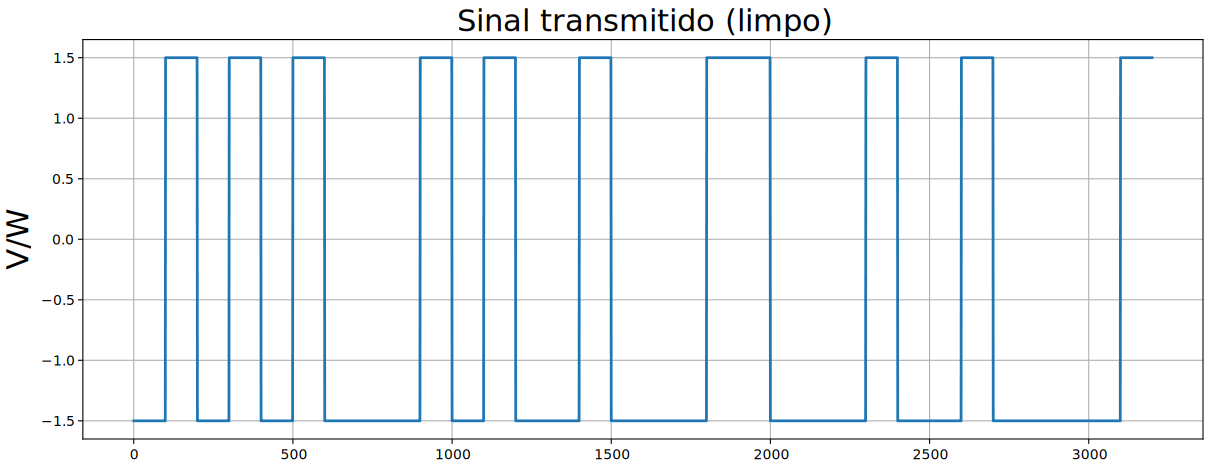
\includegraphics[width=\textwidth]{img/NRZ.png}
\caption{Sinal da modulação digital NRZ-Polar (banda-base).}
\label{fig:nrz}
\end{figure}

\begin{figure}[H]
\centering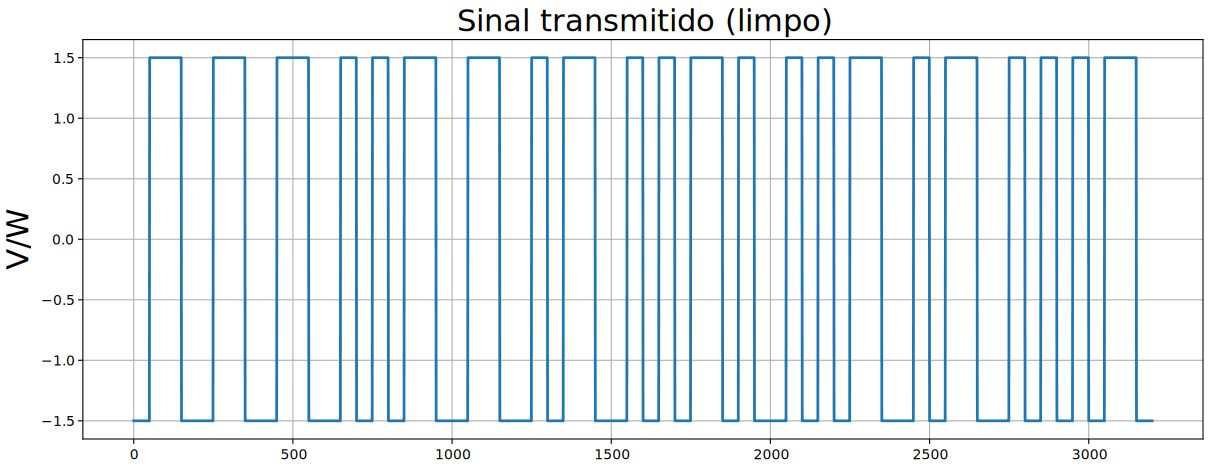
\includegraphics[width=\textwidth]{img/manchester.png}
\caption{Sinal da modulação digital Manchester (banda-base).}
\label{fig:manchester}
\end{figure}

\begin{figure}[H]
\centering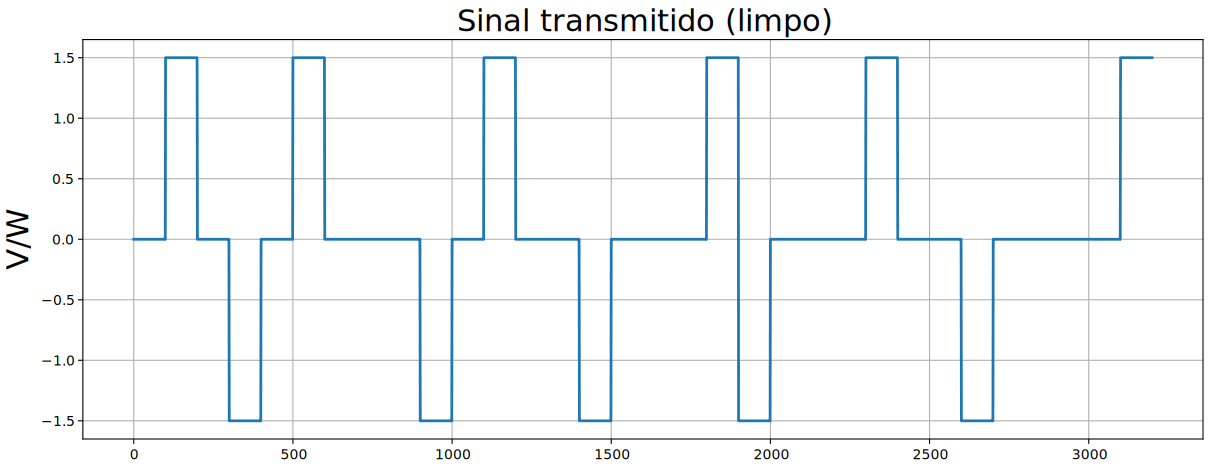
\includegraphics[width=\textwidth]{img/bipolar.png}
\caption{Sinal da modulação digital Bipolar (banda-base).}
\label{fig:bipolar}
\end{figure}

\begin{figure}[H]
\centering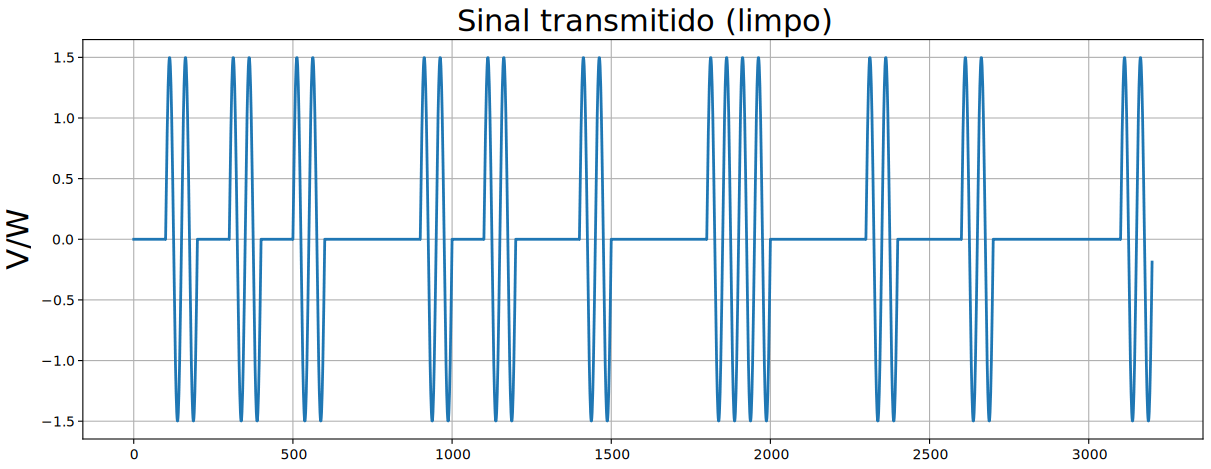
\includegraphics[width=\textwidth]{img/ASK.png}
\caption{Sinal da modulação por portadora ASK.}
\label{fig:ask}
\end{figure}

\begin{figure}[H]
\centering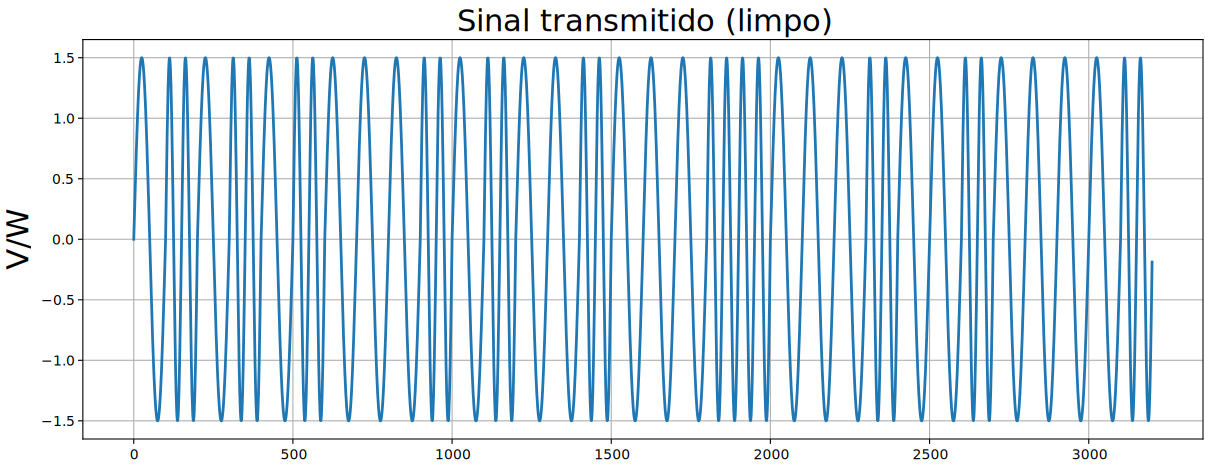
\includegraphics[width=\textwidth]{img/FSK.png}
\caption{Sinal da modulação por portadora FSK.}
\label{fig:fsk}
\end{figure}

\begin{figure}[H]
\centering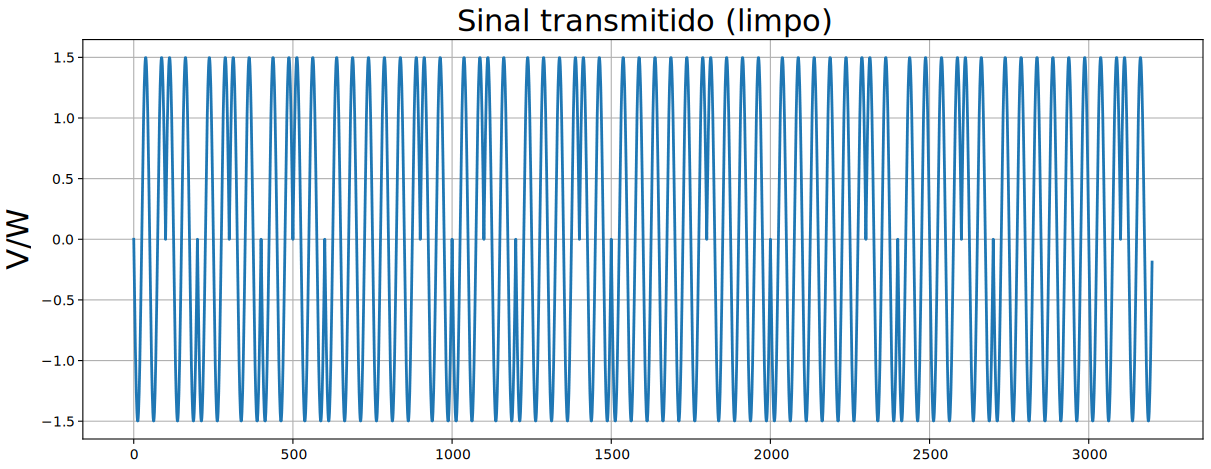
\includegraphics[width=\textwidth]{img/PSK.png}
\caption{Sinal da modulação por portadora PSK.}
\label{fig:psk}
\end{figure}

\begin{figure}[H]
\centering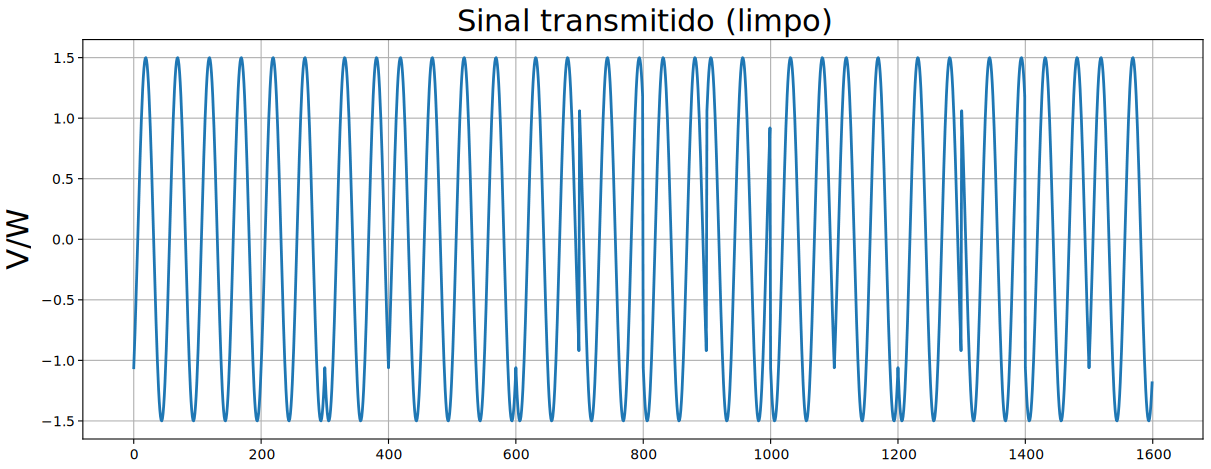
\includegraphics[width=\textwidth]{img/QPSK.png}
\caption{Sinal da modulação por portadora QPSK.}
\label{fig:qpsk}
\end{figure}

\begin{figure}[H]
\centering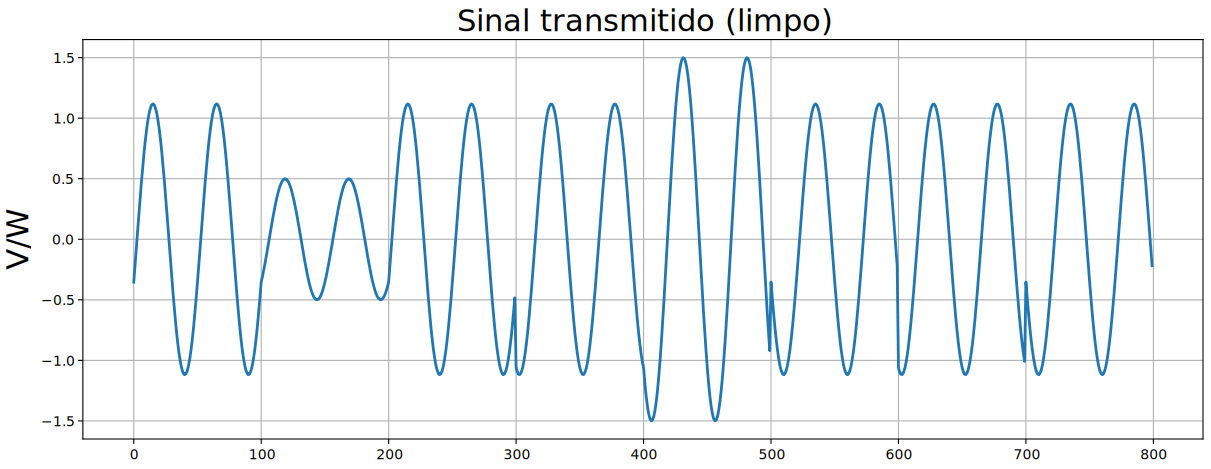
\includegraphics[width=\textwidth]{img/16QAM.png}
\caption{Sinal da modulação por portadora 16-QAM.}
\label{fig:16qam}
\end{figure}

Para o QPSK cada portadora carrega 2bits, logo o gráfico contem a metade do número de amostras e para o 16-QAM, carrega 4bits,
assim são usados um quarto do número de amostras. Na sequência segue o exemplo com ruído

\begin{figure}[h!]
    \centering 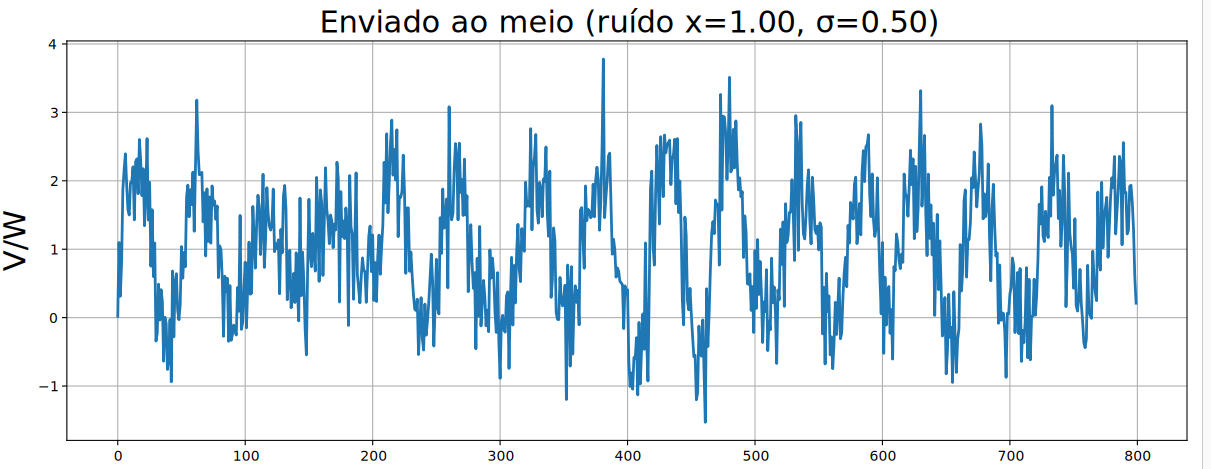
\includegraphics[width=\textwidth]{img/portadora_ruido.png}
    \caption{Portadora com Ruído: 16-QAM, $\mu = 1$, $\sigma=0.5$}
    \label{fig:portadora_ruido}
\end{figure}

\subsection{Camada de Enlace}

A camada de enlace opera sobre bits. No TX o pipeline é
\emph{payload $\rightarrow$ adiciona EDC/ECC $\rightarrow$ enquadra}; no RX, o inverso. Foram
implementados:

\begin{itemize}\itemsep1pt
    \item \textbf{Enquadramento}: (i) \emph{contagem de caracteres}, com cabeçalho de
    \textbf{16 bits} indicando o tamanho do quadro \emph{em bits} (e não em caracteres, como
    pede o enunciado); (ii) \emph{inserção de bytes} com flag \texttt{0x7E} e escape \texttt{0x7D}; (iii) \emph{inserção de bits}
    , inserindo um \texttt{0} após cinco \texttt{1} consecutivos.
    \item \textbf{Detecção (EDC)}: bit de \emph{paridade par}; \emph{checksum} por soma em
    complemento de um com \emph{carry} circular; e \textbf{CRC-32} implementado manualmente por
    divisão polinomial (gerador IEEE 802, \texttt{0x04C11DB7}).
    \item \textbf{Correção (ECC)}: código de \textbf{Hamming}, com bits de paridade nas posições
    potência de 2; no RX, a implementação localiza e corrige 1 bit invertido por quadro.
\end{itemize}


\textbf{Cenário de teste:} Foi alterado o número de amostras para 1 de forma a ficar visível o número de bits do quadro.
Valor de bits por quadro foi fixado em 8. 
Além disso, será transmitido apenas o caractere "T" por simplicidade "01010100". 

\begin{figure}[H]
\centering
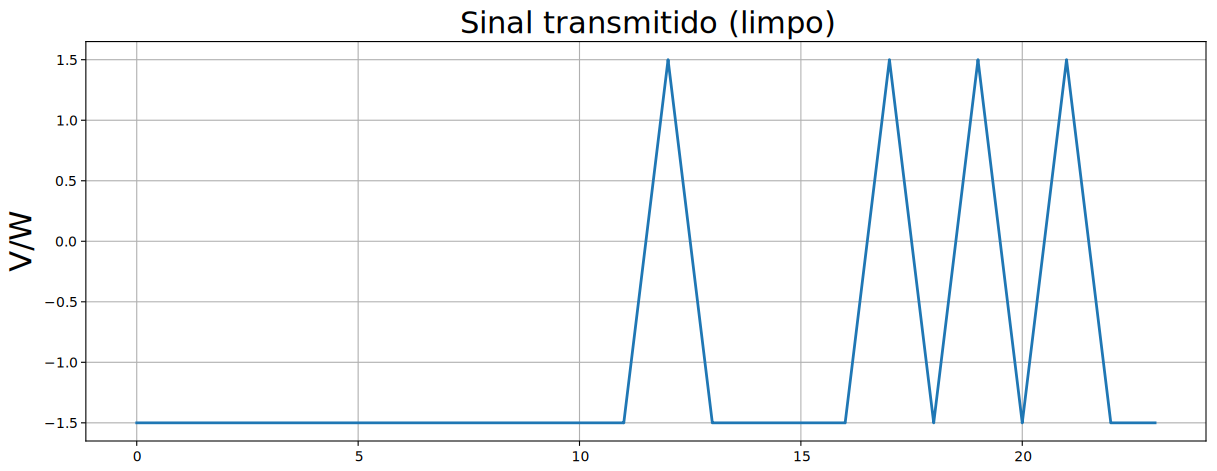
\includegraphics[width=\textwidth]{img/contagem.png}
\caption{Enquadramento por contagem de caracteres - cabeçalho de 16 bits + payload}
\label{fig:enq-contagem}
\end{figure}

\begin{figure}[H]
\centering
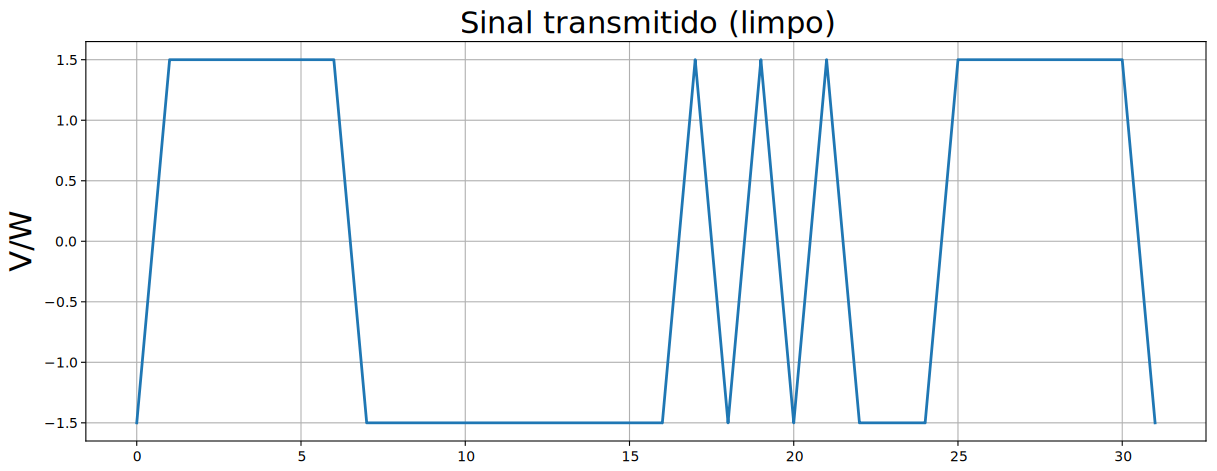
\includegraphics[width=\textwidth]{img/insertbytes.png}
\caption{Enquadramento por inserção de bytes}
\label{fig:enq-bytes}
\end{figure}

\begin{figure}[H]
\centering
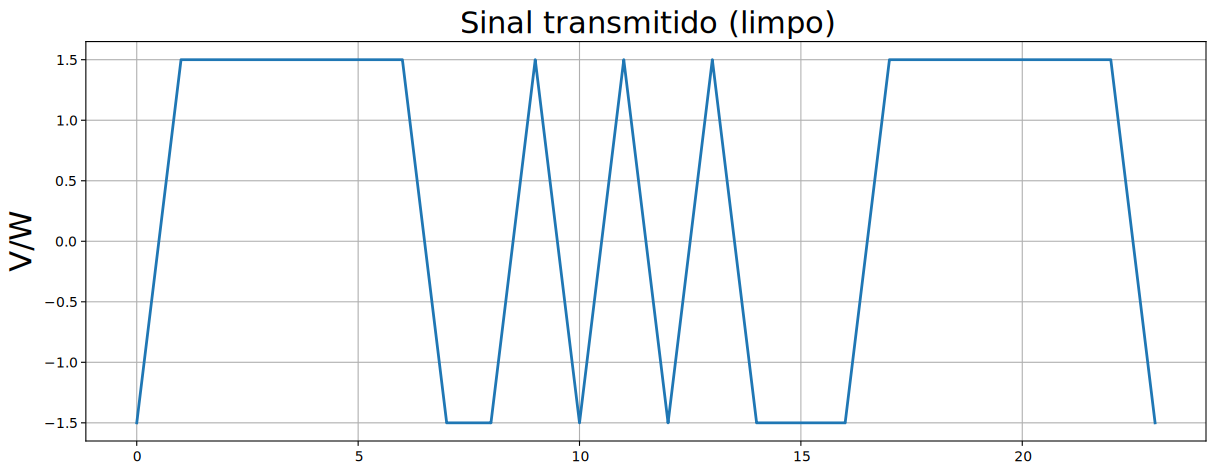
\includegraphics[width=\textwidth]{img/insertbits.png}
\caption{Enquadramento por inserção de bits}
\label{fig:enq-bits}
\end{figure}

\begin{figure}[H]
\centering
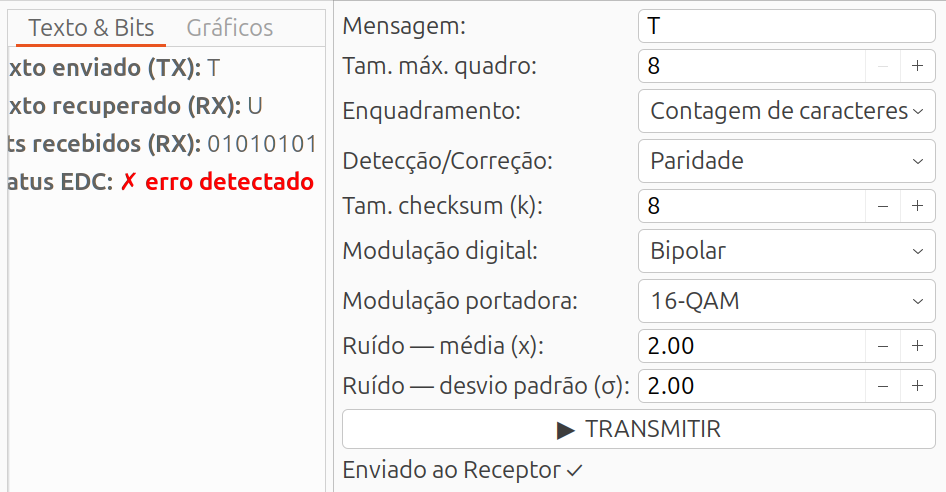
\includegraphics[width=\textwidth]{img/detecao_paridade.png}
\caption{Demonstração de detecção de erro por paridade}
\label{fig:enlace}
\end{figure}

\subsection{Meio de comunicação e ruído}

A função \texttt{aplicar\_ruido} soma a cada amostra do sinal um ruído gaussiano $n(x,\sigma)$
gerado com \texttt{random.gauss} (biblioteca padrão), com média $x$ e desvio $\sigma$
configuráveis na GUI. O ruído permite demonstrar, na prática, a atuação dos protocolos de
detecção e correção.

\subsection{Decisões de projeto e divergências do diagrama inicial}
\label{subsec:divergencias}

Durante a implementação, alguns pontos exigiram decisões de projeto, e o
produto final divergiu em alguns aspectos do diagrama inicialmente esboçado:

\begin{enumerate}\itemsep1pt
    \item \textbf{Tamanho máximo do quadro fixado em 212 bits} (\texttt{TAMANHO\_QUADRO},
    múltiplo de 8). O \emph{payload} máximo é restrito a 212 bits não o tamanho compleo do quadro.
    \item \textbf{Contagem em bits, não em caracteres.} Embora seja solicitado
    \emph{explicitamente} o enquadramento por \emph{contagem de caracteres}, implementou-se um
    cabeçalho de \textbf{16 bits} que registra o tamanho do
    quadro \emph{em bits}.
    \item \textbf{EDC ou ECC, nunca os dois simultaneamente} por quadro. A interface permite
    escolher \emph{uma} técnica de detecção \emph{ou} a correção (Hamming), tornando-os
    mutuamente exclusivos, convenção definida pelo grupo.
    \item \textbf{Meio implementado como socket TCP} (\texttt{127.0.0.1:5001}) e \textbf{GUI em
    duas instâncias} (\texttt{--modo tx} e \texttt{--modo rx}), em vez de uma janela única, 
    são duas instâncias separadas do programa.
\end{enumerate}

\subsection{Uso de Inteligência Artificial}

Por transparência, registra-se que o \textbf{GUIA\_IMPLEMENTACAO.md} (guia inicial de construção) do projeto foi
elaborado com auxílio de IA, com o intuito de \emph{deixar mais claro para o grupo} como
dividir as tarefas e qual o passo a passo de desenvolvimento, além dele o arquivo \textbf{README.md} também foi realizado da mesma forma. 
Entretanto, \textbf{toda a lógica de implementação foi desenvolvida pelo grupo}: a IA não foi utilizada para corrigir erros,
apenas para depurar e identificar possíveis falhas de lógica na implementação no caso da interface gráfica, 
corrigidas pelos próprios integrantes. Por fim, foi utilizada a IA para melhorar a construções verbal e estrutura
dos comentários dos códigos.

% ==================================================================
%  3. MEMBROS
% ==================================================================
\section{Membros e atividades}

\begin{table}[H]
\centering
\small
\begin{tabular}{@{}ll@{}}
\toprule
\textbf{Integrante} & \textbf{Atividades desenvolvidas} \\
\midrule
Luís Eduardo Curi Serra & Interface gráfica, camada física e correção de erros (Hamming, ECC). \\
Anna Luiza Novaes Jansen Silva & Transmissor, simulador e enquadramento (quadros). \\
João Pedro Borges Saraiva & Receptor e detecção de erros (paridade, checksum, CRC-32 --- EDC). \\
\bottomrule
\end{tabular}
\caption{Divisão de atividades entre os membros do grupo.}
\label{tab:membros}
\end{table}

% ==================================================================
%  4. CONCLUSÃO
% ==================================================================
\section{Conclusão}

O simulador atendeu aos requisitos do enunciado, transmitindo corretamente a mensagem através
das camadas física e de enlace e demonstrando a detecção e a correção de erros sob ruído. A
parte mais \textbf{difícil} foi o \emph{front-end} da interface gráfica, principalmente pela
falta de conhecimento prévio do grupo em GTK e pelo esforço para deixá-la minimamente estética.
A \textbf{camada física} mostrou-se objetiva e direta de implementar. Já a \textbf{camada de
enlace} foi a mais desafiadora em termos de decisões de projeto, em especial a escolha do
tamanho dos quadros e se o \emph{payload} deveria ou não ser separado dentro do quadro, além
da lógica de desenquadramento.

O trabalho \textbf{auxiliou bastante o grupo} a concretizar conceitos da
camada de enlace que, até então, eram bastante abstratos, tornando tangíveis o enquadramento e
os mecanismos de controle de erros vistos ao longo da disciplina.

% ==================================================================
%  REFERÊNCIAS
% ==================================================================
\bibliographystyle{plain}
\bibliography{bib}

\end{document}
